\documentclass[12pt,titlepage]{article}
\usepackage[margin=1.25in]{geometry}
\usepackage{graphicx,amsmath,blindtext,minted}

%% Variables definition
\newcommand{\vSubject}{Data Structure and Algorithm Practicum}
\newcommand{\vSubtitle}{Queue}
\newcommand{\vName}{Muhammad Baihaqi Aulia Asy'ari}
\newcommand{\vNIM}{2241720145}
\newcommand{\vClass}{1I}
\newcommand{\vDepartment}{Information Technology}
\newcommand{\vStudyProgram}{D4 Informatics Engineering}

%% [START] Tikz related stuff
\usepackage{tikz}
\usetikzlibrary{svg.path,calc,shapes.geometric,shapes.misc}
\tikzstyle{terminator} = [rectangle, draw, text centered, rounded corners = 1em, minimum height=2em]
\tikzstyle{preparation} = [chamfered rectangle, chamfered rectangle sep=0.75em, draw, text centered, minimum height = 2em]
\tikzstyle{process} = [rectangle, draw, text centered, minimum height=2em]
\tikzstyle{decision} = [diamond, aspect=2, draw, text centered, minimum height=2em]
\tikzstyle{data}=[trapezium, draw, text centered, trapezium left angle=60, trapezium right angle=120, minimum height=2em]
\tikzstyle{connector} = [line width=0.25mm,->]
%% [END] Tikz related stuff

%% [START] Fancy header related stuff
\usepackage{fancyhdr}
\pagestyle{fancy}
\setlength{\headheight}{15pt} % compensate fancyhdr style
\fancyhead{}
\fancyfoot{}
\fancyfoot[L]{\thepage}
\fancyfoot[R]{\textit{\vSubject - \vSubtitle}}
\renewcommand{\footrulewidth}{0.4pt}% default is 0pt, overline for footer
%% [END] Fancy header related stuff

%% [START] Custom tabular command related stuff
\usepackage{tabularx}
\newcommand{\details}[2]{
    #1 & #2  \\
}
%% [END] Custom tabular command related stuff

%% [START] Figure related stuff
\newcommand{\image}[3][1]{
    \begin{figure}[h]
        \centering
        \includegraphics[#1]{#2}
        \caption{#3}
        \label{#3}
    \end{figure}
}
%% [END] Figure related stuff

%%
\usepackage{pgf-umlcd}

\renewcommand{\umldrawcolor}{black}
\renewcommand{\umlfillcolor}{white}
%%

%% [BEGIN] Custom enumerator
\usepackage{enumitem}
%% [END] Custom enumerator

%% [BEGIN] Paragraph indent
\usepackage{indentfirst}
%% [END] Paragraph indent

\begin{document}
\begin{titlepage}
    \centering
    \vfill
    {\bfseries\LARGE
        \vSubject\\
        \vskip0.25cm
        \vSubtitle
    }
    \vfill
    \includegraphics[width=6cm]{images/polinema-logo.png}
    \vfill
    {
        \textbf{Name}\\
        \vName\\
        \vskip0.5cm
        \textbf{NIM}\\
        \vNIM\\
        \vskip0.5cm
        \textbf{Class}\\
        \vClass\\
        \vskip0.5cm
        \textbf{Department}\\
        \vDepartment\\
        \vskip0.5cm
        \textbf{Study Program}\\
        \vStudyProgram
    }
\end{titlepage}

\newpage

\setcounter{section}{1}
\subsection{Learning Objective}
After finishing this topic, students must be able to:
\begin{enumerate}
    \item Understand the basic concept of Queue
    \item Understand the basic operation of Queue
    \item Implement the Queue concept as well as the operation in a program by using Java
\end{enumerate}

\subsection{Lab Activities 1}
\subsubsection{Steps}
\begin{enumerate}
    \item We will create a program based on this following class diagram
    \mbox{}\\
    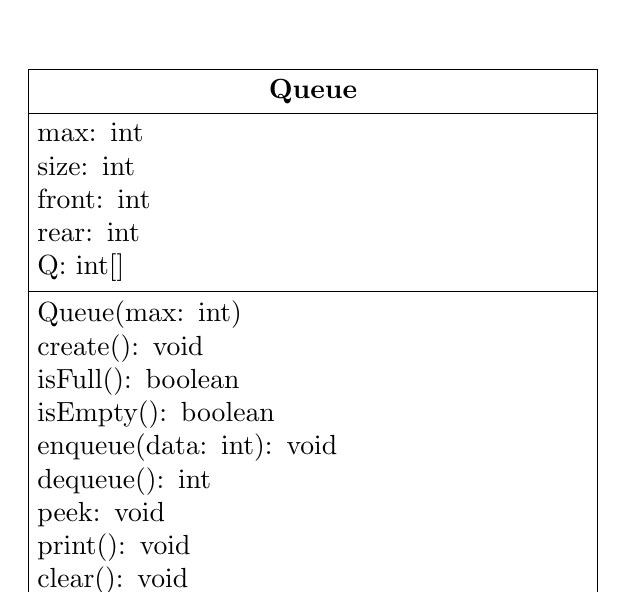
\begin{tikzpicture}
        \begin{class}[text width=7cm]{Queue}{0,0}
            \attribute{max: int}
            \attribute{size: int}
            \attribute{front: int}
            \attribute{rear: int}
            \attribute{Q: int[]}
            \operation{Queue(max: int)}
            \operation{create(): void}
            \operation{isFull(): boolean}
            \operation{isEmpty(): boolean}
            \operation{enqueue(data: int): void}
            \operation{dequeue(): int}
            \operation{peek: void}
            \operation{print(): void}
            \operation{clear(): void}
        \end{class}
    \end{tikzpicture}
    \mbox{}\\
    \item Create a new project named \textbf{Jobsheet8}, create a new package with name \textbf{practicum1}. After that, create a new class \textbf{Queue}
    \item Add max, size, front,rear and Q as its attributes based on the class diagram above.
    \item Add a constructor with parameter and method create as illustration below.
    \begin{minted}[autogobble,breaklines]{java}
        public Queue(int n) {
            max = 4;
            Create();
        }
    \end{minted}
    Within the constructor, there is a code to execute \textbf{create()}. then we make the create function
    \begin{minted}[autogobble,breaklines]{java}
        public void Create() {
            Q = new int[max];
            size = 0;
            front = rear = -1;
        }
    \end{minted}
    \item Create a method isEmpty with boolean as its return data type. We use this function to identify whether a queue is empty or not
    \begin{minted}[autogobble,breaklines]{java}
        public boolean isEmpty() {
            if (size == 0) {
                return true;
            } else {
                return false;
            }
        }
    \end{minted}
    \item Create a method isFull with boolean as its return data type. We use this function to identify whether a queue is full or not
    \begin{minted}[autogobble,breaklines]{java}
        public boolean isFull() {
            if (size == max) {
                return true;
            } else {
                return false;
            }
        }
    \end{minted}
    \item Create \textbf{peek()} with void as its return type to display the data at the beginning of the queue
    \begin{minted}[autogobble,breaklines]{java}
        public void peek() {
            if (!isEmpty()) {
                System.out.println("The first element : " + Q[front]);
            } else {
                System.out.println("Queue is still empty");
            }
        }
    \end{minted}
    \item Create \textbf{print()} with void as its return type to display the data from the beginning until the end of the queue
    \begin{minted}[autogobble,breaklines]{java}
        public void print() {
            if (!isEmpty()) {
                System.out.println("Queue is still empty");
            } else {
                int i = front;
                while (i != rear) {
                    System.out.println(Q[i] + " ");
                    i = (i+1) % max;
                }
                System.out.println(Q[i] + " ");
                System.out.println("Element amount : " + size);
            }
        }
    \end{minted}
    \item Create \textbf{clear()} with void as its return type to remove all data in a queue
    \begin{minted}[autogobble,breaklines]{java}
        public void clear() {
            if (!isEmpty()) {
                front = rear = -1;
                size = 0;
                System.out.println("Queue has been cleared successfully");
            } else {
                System.out.println("Queue is still empty");
            }
        }
    \end{minted}
    \item. Next up, we make a new method \textbf{enqueue()} to insert a new data in a queue that has integer datatype as its parameter
    \begin{minted}[autogobble,breaklines]{java}
        public void enqueue(int data) {
            if (isFull()) {
                System.out.println("Queue is already full");
            } else {
                if (isEmpty()) {
                    front = rear = 0;
                } else {
                    if (rear == max - 1) {
                        rear = 0;
                    } else {
                        rear++;
                    }
                }
                Q[rear] = data;
                size++;
            }
        }
    \end{minted}
    \item. Create method \textbf{dequeue()} with integer as its return type. We will need this function whenever we want to remove the last data inside the queue
    \begin{minted}[autogobble,breaklines]{java}
        public int dequeue() {
            int data = 0;
            if (isEmpty()) {
                System.out.println("Queue is still empty");
            } else {
                data = Q[front];
                size--;
                if (isEmpty()) {
                    front = rear = -1;
                } else {
                    if (front == max - 1) {
                        front = 0;
                    } else {
                        front++;
                    }
                }
            }
            return data;
        }
    \end{minted}
    \item. Next, we create a new class named \textbf{QueueMain} still at the same package \textbf{Practicum1}. To create a menu with void return type to allow user choose which function to be executed when the program runs
    \begin{minted}[autogobble,breaklines]{java}
        public static void menu() {
            System.out.println("Choose menu: ");
            System.out.println("1. Enqueue");
            System.out.println("2. Dequeue");
            System.out.println("3. Print");
            System.out.println("4. Peek");
            System.out.println("5. Clear");
            System.out.println("================================");
        }
    \end{minted}
    \item. Create a main function, and declare the Scanner object with name \textbf{sc}
    \item. Create \textbf{n} variable to store input of how many elements that can be stored within the queue
    \begin{minted}[autogobble,breaklines]{java}
        Scanner sc = new Scanner(System.in);
        System.out.print("Insert maximum queue : ");
        int n = sc.nextInt();
    \end{minted}
    \item. Instantiate the Queue object with name \textbf{Q} and set the parameter \textbf{n} as its queue length
    \begin{minted}[autogobble,breaklines]{java}
        Queue Q = new Queue(n);
    \end{minted}
    \item. Declare the input of menu selected by user
    \item. Loop with do-while to run the program based on the given input. Inside the loop, there is a switch case condition to manipulate queue based on the given input
    \begin{minted}[autogobble,breaklines]{java}
        int choose;
        do {
            menu();
            choose = sc.nextInt();
            switch (choose) {
                case 1:
                    System.out.print("Insert new data: ");
                    int newData = sc.nextInt();
                    Q.enqueue(newData);
                    break;
                
                case 2:
                    int removeData = Q.dequeue();
                    if (removeData != 0) {
                        System.out.println("Data removed : " + removeData);
                        break;
                    }
            
                case 3 :
                    Q.print();
                    break;
                
                case 4:
                    Q.peek();
                    break;

                case 5:
                    Q.clear();
                    break;
            }
        } while (choose <= 5 && choose >= 1);
    \end{minted}
    \item. Compile the program and run the \textbf{QueueMain} class. And observe the result
    \begin{minted}[autogobble,breaklines]{java}
        package practicum1;

        public class Queue {
            int max, size, front, rear;
            int[] Q;
            
            public Queue(int n) {
                max = n;
                create();
            }

            public void create() {
                Q = new int[max];
                size = 0;
                front = rear = -1;
            }

            public boolean isEmpty() {
                if (size == 0) {
                    return true;
                } else {
                    return false;
                }
            }

            public boolean isFull() {
                if (size == max) {
                    return true;
                } else {
                    return false;
                }
            }

            public void peek() {
                if (!isEmpty()) {
                    System.out.println("The first element : " + Q[front]);
                } else {
                    System.out.println("Queue is still empty");
                }
            }

            public void print() {
                if (!isEmpty()) {
                    System.out.println("Queue is still empty");
                } else {
                    int i = front;
                    while (i != rear) {
                        System.out.println(Q[i] + " ");
                        i = (i+1) % max;
                    }
                    System.out.println(Q[i] + " ");
                    System.out.println("Element amount : " + size);
                }
            }

            public void clear() {
                if (!isEmpty()) {
                    front = rear = -1;
                    size = 0;
                    System.out.println("Queue has been cleared successfully");
                } else {
                    System.out.println("Queue is still empty");
                }
            }

            public void enqueue(int data) {
                if (isFull()) {
                    System.out.println("Queue is already full");
                } else {
                    if (isEmpty()) {
                        front = rear = 0;
                    } else {
                        if (rear == max - 1) {
                            rear = 0;
                        } else {
                            rear++;
                        }
                    }
                    Q[rear] = data;
                    size++;
                }
            }

            public int dequeue() {
                int data = 0;
                if (isEmpty()) {
                    System.out.println("Queue is still empty");
                } else {
                    data = Q[front];
                    size--;
                    if (isEmpty()) {
                        front = rear = -1;
                    } else {
                        if (front == max - 1) {
                            front = 0;
                        } else {
                            front++;
                        }
                    }
                }
                return data;
            }
        }
    \end{minted}

    \begin{minted}[autogobble,breaklines]{java}
        package practicum1;

        import java.util.Scanner;

        public class QueueMain {
            public static void menu() {
                System.out.println("Choose menu: ");
                System.out.println("1. Enqueue");
                System.out.println("2. Dequeue");
                System.out.println("3. Print");
                System.out.println("4. Peek");
                System.out.println("5. Clear");
                System.out.println("================================");
            }

            public static void main(String[] args) {
                Scanner sc = new Scanner(System.in);
                System.out.print("Insert maximum queue : ");
                int n = sc.nextInt();

                Queue Q = new Queue(n);

                int choose;
                do {
                    menu();
                    choose = sc.nextInt();
                    switch (choose) {
                        case 1:
                            System.out.print("Insert new data: ");
                            int newData = sc.nextInt();
                            Q.enqueue(newData);
                            break;
                        
                        case 2:
                            int removeData = Q.dequeue();
                            if (removeData != 0) {
                                System.out.println("Data removed : " + removeData);
                                break;
                            }
                    
                        case 3 :
                            Q.print();
                            break;
                        
                        case 4:
                            Q.peek();
                            break;

                        case 5:
                            Q.clear();
                            break;
                    }
                } while (choose <= 5 && choose >= 1);

                sc.close();
            }
        }
    \end{minted}
\end{enumerate}

\subsubsection{Result}
Check if the result match with following image:
\begin{minted}[autogobble,breaklines,linenos]{text}
    PS D:\Kuliah>  d:; cd 'd:\Kuliah'; & 'C:\Program Files\Java\jdk-18.0.2.1\bin\java.exe' '-XX:+ShowCodeDetailsInExceptionMessages' '-cp' 'C:\Users\G4CE-PC\AppData\Roaming\Code\User\workspaceStorage\ 80d97a47d24665dc0bce7ab1e048ecbd\redhat.java\jdt_ws\Kuliah_28156aa7\bin' 'QueueMain' 
    Insert maximum queue : 4
    Choose menu: 
    1. Enqueue
    2. Dequeue
    3. Print
    4. Peek
    5. Clear
    ================================
    1
    Insert new data: 15
    Choose menu: 
    1. Enqueue
    2. Dequeue
    3. Print
    4. Peek
    5. Clear
    ================================
    1
    Insert new data: 31
    Choose menu: 
    1. Enqueue
    2. Dequeue
    3. Print
    4. Peek
    5. Clear
    ================================
    4
    The first element : 15
    Choose menu:
    1. Enqueue
    2. Dequeue
    3. Print
    4. Peek
    5. Clear
    ================================
\end{minted}

\subsubsection{Questions}
\begin{enumerate}
    \item In method create(), why is the front and rear attribute has initial value with 1 and not 0?
    \mbox{}\\
    \texttt{Answer: }
    \mbox{}\\
    The front and rear attribute is initialized with the number -1 to indicate that the queue is empty and there is no front index or rear index yet. This would make the array out of bound error when it apply to the array.
    \item In method enqueue(), please explain the usage of this following code
    \begin{minted}[autogobble,breaklines]{java}
        if (rear == max - 1) {
            rear = 0;
        }
    \end{minted}
    \texttt{Answer: }
    \mbox{}\\
    The if condition checks for the rear index. When it reach the maximum index of the queue, it will reset the rear index to 0. If the queue is full nothing would happend. But when the queue has more room, because the rear index has been reset to 0, the data will be insert at the rear which is at the first index.
    \item Observe enqueue() method, which line of code indicates that the new data will be stored in last position of the queue?
    \mbox{}\\
    \texttt{Answer: }
    \begin{minted}[autogobble,breaklines]{java}
        Q[rear] = data;
    \end{minted}
    \item Observe dequeue() method, which line of code indicates that the data is removed in the first position of the queue?
    \mbox{}\\
    \texttt{Answer: }
    \begin{minted}[autogobble,breaklines]{java}
        data = Q[front];
    \end{minted}
    \item In dequeue method(), explain the usage of these codes !
    \begin{minted}[autogobble,breaklines]{java}
        if (front == max - 1) {
            front = 0;
        }
    \end{minted}
    \texttt{Answer: }
    \mbox{}\\
    The if condition checks for the front index. When it reach the maximum index of the queue, it will reset the front index to 0. If the queue is full nothing would happend. But when the queue has more room, because the front index has been reset to 0, the data will be drop at the front which is at the first index.
    \item In method print(), why the loop process has \textbf{int i = 0} instead of int \textbf{i=front}?
    \texttt{Answer: }
    \mbox{}\\
    Because the the first element of a queue doesn't necessarily start at the index 0. That is why queue keep the index of the first element instead of constantly rewriting the array as such that the first element is at the first index of the array.
    \item In method print(), please explain why we insert this code in our program?
    \begin{minted}[autogobble,breaklines]{java}
        i = (i + 1) % max;
    \end{minted}
    \texttt{Answer: }
    \mbox{}\\
    The code is used to increment the i as such that the i will only cycle trough the index up to the maximum index and then return to 0 to then cycle again.
\end{enumerate}

\subsection{Lab Activities 2}
In this lab activity, we will create a train ticket payment simple program with implementing the properties adjusted in railway stations environment
\subsubsection{Steps}
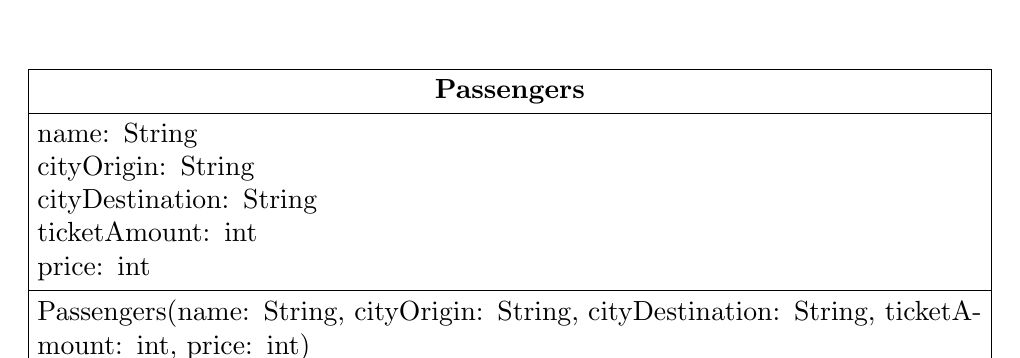
\begin{tikzpicture}
    \begin{class}[text width=12cm]{Passengers}{0,0}
        \attribute{name: String}
        \attribute{cityOrigin: String}
        \attribute{cityDestination: String}
        \attribute{ticketAmount: int}
        \attribute{price: int}
        \operation{Passengers(name: String, cityOrigin: String, cityDestination: String, ticketAmount: int, price: int)}
    \end{class}
\end{tikzpicture}

\begin{enumerate}
    \item Based on above class diagram, we will create a program written in Java
    \item Create a new package named \textbf{Practicum2} and create a new class named \textbf{Passengers}
    \item Add attributes for Passengers based on above class diagram, add the constructor as well
    \item Copy the program code written in \textbf{Queue} in 1\textsuperscript{st} Lab Activities to be reused in this package. We will need to modify the class, since the stored value in 1st lab activity is in integer data type, but we need it to store an object
    \item Modify the class \textbf{Queue}, we change the data type \textbf{int[] Q} into \textbf{Passenger[] Q}. Since this case we will need to store Passenger object in the queue. In addition, we will need to modify \textbf{attributes, create(), enqueue(), and dequeue()}
    \begin{minted}[autogobble,breaklines]{java}
        int max, size, front, rear;
        Passengers[] Q;
        
        public void create() {
            Q = new Passengers[max];
            size = 0;
            front = rear = -1;
        }

        public void enqueue(Passengers data) {
            if (isFull()) {
                System.out.println("Queue is already full");
            } else {
                if (isEmpty()) {
                    front = rear = 0;
                } else {
                    if (rear == max - 1) {
                        rear = 0;
                    } else {
                        rear++;
                    }
                }
                Q[rear] = data;
                size++;
            }
        }

        public Passengers dequeue() {
            Passengers data = new Passengers("", "", "", 0, 0);
            if (isEmpty()) {
                System.out.println("Queue is still empty");
            } else {
                data = Q[front];
                size--;
                if (isEmpty()) {
                    front = rear = -1;
                } else {
                    if (front == max - 1) {
                        front = 0;
                    } else {
                        front++;
                    }
                }
            }
            return data;
        }
    \end{minted}
    \item Because one element in queue holds some information (name, cityOrigin, cityDestination, ticketAmount, price), we are needed to display all of that information. This leads to modifying the \textbf{peek() and print()} as well
    \begin{minted}[autogobble,breaklines]{java}
        public void peek() {
            if (!isEmpty()) {
                System.out.println("The first element : " + Q[front].name + " " + Q[front].cityOrigin + " " + Q[front].cityDestination + " " + Q[front].ticketAmount + " " + Q[front].price);
            } else {
                System.out.println("Queue is still empty");
            }
        }

        public void print() {
            if (isEmpty()) {
                System.out.println("Queue is still empty");
            } else {
                int i = front;
                while (i != rear) {
                    System.out.println("The first element : " + Q[i].name + " " + Q[i].cityOrigin + " " + Q[i].cityDestination + " " + Q[i].ticketAmount + " " + Q[i].price);
                    i = (i+1) % max;
                }
                System.out.println(Q[i].name + " " + Q[i].cityOrigin + " " + Q[i].cityDestination + " " + Q[i].ticketAmount + " " + Q[i].price);
                System.out.println("Element amount : " + size);
            }
        }
    \end{minted}
    \item Next, create a new class named \textbf{QueueMain} within the \textbf{Practicum2} package. Create \textbf{menu()} to provide menu options and allow the user to choose the menu when the program runs
    \begin{minted}[autogobble,breaklines]{java}
        public static void menu() {
            System.out.println("Choose menu: ");
            System.out.println("1. Queue");
            System.out.println("2. Dequeue");
            System.out.println("3. Check first queue");
            System.out.println("4. Check all queue");
            System.out.println("================================");
        }
    \end{minted}
    \item Create \textbf{main method} in the \textbf{QueueMain}, and declare the Scanner object with name \textbf{sc}
    \item Create \textbf{max} variable to define the capacity of the queue. After that, instantiate queue object with name \textbf{queuePassenger} with its parameter is \textbf{max}
    \begin{minted}[autogobble,breaklines]{java}
        System.out.print("Insert maximum queue : ");
        int max = sc.nextInt();
        Queue queuePassenger = new Queue(max);
    \end{minted}
    \item Declare a variable named \textbf{choose} with integer as its datatype to get which option did the user choose.
    \item Add these following codes to loops menu options according to given input by the user.
    \begin{minted}[autogobble,breaklines]{java}
        int choose;
        do {
            menu();
            choose = sc.nextInt();
            switch (choose) {
                case 1:
                    System.out.print("Name: ");
                    sc.nextLine();
                    String name = sc.nextLine();
                    System.out.print("City origin: ");
                    String cityOrigin = sc.nextLine();
                    System.out.print("City Destination: ");
                    String cityDestination = sc.nextLine();
                    System.out.print("Ticket Amount: ");
                    int ticket = sc.nextInt();
                    System.out.print("Price: ");
                    int price = sc.nextInt();
                    Passengers p = new Passengers(name, cityOrigin, cityDestination, ticket, price);
                    sc.nextLine();
                    queuePassenger.enqueue(p);
                    break;
            
                case 2:
                    Passengers data = queuePassenger.dequeue();
                    if (!"".equals(data.name) && !"".equals(data.cityOrigin) && !"".equals(data.cityDestination) && !"".equals(data.ticketAmount) && !"".equals(data.price)) {
                        System.out.println("Data removed : " + data.name + " " + data.cityOrigin + " " + data.cityDestination + " " + data.ticketAmount + " " + data.price);
                        break;
                    }
                
                case 3:
                    queuePassenger.peek();
                    break;
                
                case 4:
                    queuePassenger.print();
                    break;
                
                case 5:
                    queuePassenger.clear();
                    break;
            }
        } while (choose <= 4 && choose >= 1);
    \end{minted}
    \item Compile the program and run the \textbf{QueueMain} class. And observe the result
    \begin{minted}[autogobble,breaklines]{java}
        package practicum2;

        public class Passengers {
            String name,
            cityOrigin,
            cityDestination;
            
            int ticketAmount,
            price;

            public Passengers(String name, String cityOrigin, String cityDestination, int ticketAmount, int price) {
                this.name = name;
                this.cityOrigin = cityOrigin;
                this.cityDestination = cityDestination;
                this.ticketAmount = ticketAmount;
                this.price = price;
            }
        }
    \end{minted}

    \begin{minted}[autogobble,breaklines]{java}
        package practicum2;
        
        public class Queue {
            int max, size, front, rear;
            Passengers[] Q;
            
            public Queue(int n) {
                max = n;
                create();
            }

            public void create() {
                Q = new Passengers[max];
                size = 0;
                front = rear = -1;
            }

            public boolean isEmpty() {
                if (size == 0) {
                    return true;
                } else {
                    return false;
                }
            }

            public boolean isFull() {
                if (size == max) {
                    return true;
                } else {
                    return false;
                }
            }

            public void peek() {
                if (!isEmpty()) {
                    System.out.println("The first element : " + Q[front].name + " " + Q[front].cityOrigin + " " + Q[front].cityDestination + " " + Q[front].ticketAmount + " " + Q[front].price);
                } else {
                    System.out.println("Queue is still empty");
                }
            }

            public void print() {
                if (isEmpty()) {
                    System.out.println("Queue is still empty");
                } else {
                    int i = front;
                    while (i != rear) {
                        System.out.println("The first element : " + Q[i].name + " " + Q[i].cityOrigin + " " + Q[i].cityDestination + " " + Q[i].ticketAmount + " " + Q[i].price);
                        i = (i+1) % max;
                    }
                    System.out.println(Q[i].name + " " + Q[i].cityOrigin + " " + Q[i].cityDestination + " " + Q[i].ticketAmount + " " + Q[i].price);
                    System.out.println("Element amount : " + size);
                }
            }

            public void clear() {
                if (!isEmpty()) {
                    front = rear = -1;
                    size = 0;
                    System.out.println("Queue has been cleared successfully");
                } else {
                    System.out.println("Queue is still empty");
                }
            }

            public void enqueue(Passengers data) {
                if (isFull()) {
                    System.out.println("Queue is already full");
                } else {
                    if (isEmpty()) {
                        front = rear = 0;
                    } else {
                        if (rear == max - 1) {
                            rear = 0;
                        } else {
                            rear++;
                        }
                    }
                    Q[rear] = data;
                    size++;
                }
            }

            public Passengers dequeue() {
                Passengers data = new Passengers("", "", "", 0, 0);
                if (isEmpty()) {
                    System.out.println("Queue is still empty");
                } else {
                    data = Q[front];
                    size--;
                    if (isEmpty()) {
                        front = rear = -1;
                    } else {
                        if (front == max - 1) {
                            front = 0;
                        } else {
                            front++;
                        }
                    }
                }
                return data;
            }
        }
    \end{minted}

    \begin{minted}[autogobble,breaklines]{java}
        package practicum2;

        import java.util.Scanner;

        public class QueueMain {
            public static void menu() {
                System.out.println("Choose menu: ");
                System.out.println("1. Queue");
                System.out.println("2. Dequeue");
                System.out.println("3. Check first queue");
                System.out.println("4. Check all queue");
                System.out.println("================================");
            }

            public static void main(String[] args) {
                Scanner sc = new Scanner(System.in);

                System.out.print("Insert maximum queue : ");
                int max = sc.nextInt();
                Queue queuePassenger = new Queue(max);

                int choose;
                do {
                    menu();
                    choose = sc.nextInt();
                    switch (choose) {
                        case 1:
                            System.out.print("Name: ");
                            sc.nextLine();
                            String name = sc.nextLine();
                            System.out.print("City origin: ");
                            String cityOrigin = sc.nextLine();
                            System.out.print("City Destination: ");
                            String cityDestination = sc.nextLine();
                            System.out.print("Ticket Amount: ");
                            int ticket = sc.nextInt();
                            System.out.print("Price: ");
                            int price = sc.nextInt();
                            Passengers p = new Passengers(name, cityOrigin, cityDestination, ticket, price);
                            sc.nextLine();
                            queuePassenger.enqueue(p);
                            break;
                    
                        case 2:
                            Passengers data = queuePassenger.dequeue();
                            if (!"".equals(data.name) && !"".equals(data.cityOrigin) && !"".equals(data.cityDestination) && !"".equals(data.ticketAmount) && !"".equals(data.price)) {
                                System.out.println("Data removed : " + data.name + " " + data.cityOrigin + " " + data.cityDestination + " " + data.ticketAmount + " " + data.price);
                                break;
                            }
                        
                        case 3:
                            queuePassenger.peek();
                            break;
                        
                        case 4:
                            queuePassenger.print();
                            break;
                        
                        case 5:
                            queuePassenger.clear();
                            break;
                    }
                } while (choose <= 4 && choose >= 1);

                sc.close();
            }
        }
    \end{minted}
\end{enumerate}

\subsubsection{Result}
Check if the result match with following image:
\begin{minted}[autogobble,breaklines,linenos]{text}
    PS D:\Kuliah\Smt 2\Algoritma dan Struktur Data\Praktikum\Week 10\Queue>  d:; cd 'd:\Kuliah\Smt 2\Algoritma dan Struktur Data\Praktikum\Week 10\Queue'; & 'C:\Program Files\Java\jdk-18.0.2.1\bin\java.exe' '-XX:+ShowCodeDetailsInExceptionMessages' '-cp' 'D:\Kuliah\Smt 2\Algoritma dan Struktur Data\Praktikum\Week 10\Queue\bin' 'practicum2.QueueMain' 
    Insert maximum queue : 5
    Choose menu: 
    1. Queue
    2. Dequeue
    3. Check first queue
    4. Check all queue
    ================================
    1
    Name: Angga
    City origin: Solo
    City Destination: Sidoarjo
    Ticket Amount: 2
    Price: 176000
    Choose menu: 
    1. Queue
    2. Dequeue
    3. Check first queue
    4. Check all queue
    ================================
    1
    Name: Fadin
    City origin: Banyuwangi
    City Destination: Bandung
    Ticket Amount: 1
    Price: 65000
    Choose menu: 
    1. Queue
    2. Dequeue
    3. Check first queue
    4. Check all queue
    ================================
    3
    The first element : Angga Solo Sidoarjo 2 176000
\end{minted}

\subsubsection{Questions}
\begin{enumerate}
    \item In Queue Class, what’s the function of this program code in method Dequeue?
    \begin{minted}[autogobble,breaklines]{java}
       Passenger data = new Passenger("", "", "", 0, 0);
    \end{minted}
    \texttt{Answer: }
    \mbox{}\\
    It's used to insert a temporary empty object.
    \item In previous number, if the program code changed to Passenger data = new Passenger() What will happen?
    \mbox{}\\
    \texttt{Answer: }
    \mbox{}\\
    Java return an error for an undefined constructor.
    \item Show the program code used for displaying the data retrieved / removed from the queue!
    \mbox{}\\
    \texttt{Answer: }
    \begin{minted}[autogobble,breaklines]{java}
        public Passengers dequeue() {
            Passengers data = new Passengers("", "", "", 0, 0);
            if (isEmpty()) {
                System.out.println("Queue is still empty");
            } else {
                data = Q[front];
                size--;
                if (isEmpty()) {
                    front = rear = -1;
                } else {
                    if (front == max - 1) {
                        front = 0;
                    } else {
                        front++;
                    }
                }
            }
            return data;
        }
    \end{minted}
    \item Modify the program by adding a method named \textbf{peekRear()} in Queue class to check the last position within the queue. Add a menu for the user to perform and explore your program as well
    \mbox{}\\
    \texttt{Answer: }
    \begin{minted}[autogobble,breaklines]{java}
        public void peekRear() {
            if (!isEmpty()) {
                System.out.println("The last element : " + Q[rear].name + " " + Q[rear].cityOrigin + " " + Q[rear].cityDestination + " " + Q[rear].ticketAmount + " " + Q[rear].price);
            } else {
                System.out.println("Queue is still empty");
            }
        }
    \end{minted}
    \item Ensure that the \textbf{peekRear()} function can be executed inside the program
    \mbox{}\\
    \texttt{Answer: }
    \begin{minted}[autogobble,breaklines]{java}
        public static void menu() {
            System.out.println("Choose menu: ");
            System.out.println("1. Queue");
            System.out.println("2. Dequeue");
            System.out.println("3. Check first queue");
            System.out.println("4. Check last queue");
            System.out.println("5. Check all queue");
            System.out.println("================================");
        }
    \end{minted}
    \begin{minted}[autogobble,breaklines]{java}
        switch (choose) {
            case 1:
                System.out.print("Name: ");
                sc.nextLine();
                String name = sc.nextLine();
                System.out.print("City origin: ");
                String cityOrigin = sc.nextLine();
                System.out.print("City Destination: ");
                String cityDestination = sc.nextLine();
                System.out.print("Ticket Amount: ");
                int ticket = sc.nextInt();
                System.out.print("Price: ");
                int price = sc.nextInt();
                Passengers p = new Passengers(name, cityOrigin, cityDestination, ticket, price);
                sc.nextLine();
                queuePassenger.enqueue(p);
                break;
        
            case 2:
                Passengers data = queuePassenger.dequeue();
                if (!"".equals(data.name) && !"".equals(data.cityOrigin) && !"".equals(data.cityDestination) && !"".equals(data.ticketAmount) && !"".equals(data.price)) {
                    System.out.println("Data removed : " + data.name + " " + data.cityOrigin + " " + data.cityDestination + " " + data.ticketAmount + " " + data.price);
                    break;
                }
            
            case 3:
                queuePassenger.peek();
                break;
            
            case 4:
                queuePassenger.peekRear();
                break;
            
            case 5:
                queuePassenger.print();
                break;
            
            case 6:
                queuePassenger.clear();
                break;
        }
    \end{minted}
\end{enumerate}

\subsection{Assignments}
\begin{enumerate}
    \item Add these 2 methods in \textbf{Queue} class in 1\textsuperscript{st} practicum
    \item Make a queue program for students when they need the signs for their KRS by the DPA. If the student is in queue, they will be required to fill in some information as follows:
    \mbox{}\\
    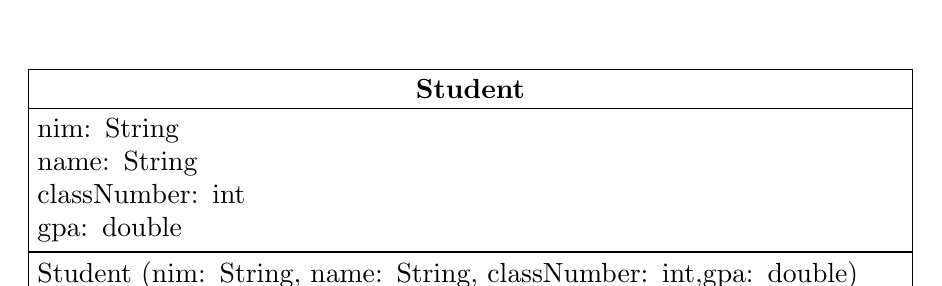
\begin{tikzpicture}
        \begin{class}[text width=11cm]{Student}{0,0}
            \attribute{nim: String}
            \attribute{name: String}
            \attribute{classNumber: int}
            \attribute{gpa: double}
            \operation{Student (nim: String, name: String, classNumber: int,gpa: double)}
        \end{class}
    \end{tikzpicture}
    \mbox{}\\
    Queue Class diagram:
    \mbox{}\\
    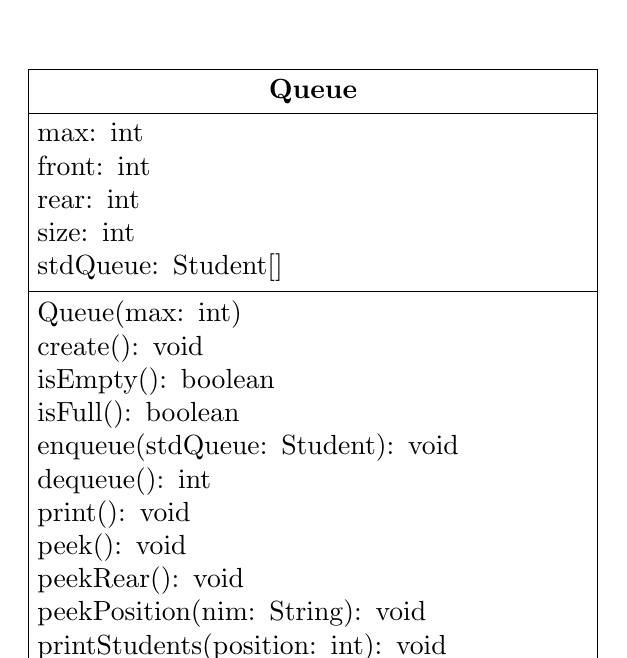
\begin{tikzpicture}
        \begin{class}[text width=7cm]{Queue}{0,0}
            \attribute{max: int}
            \attribute{front: int}
            \attribute{rear: int}
            \attribute{size: int}
            \attribute{stdQueue: Student[]}
            \operation{Queue(max: int)}
            \operation{create(): void}
            \operation{isEmpty(): boolean}
            \operation{isFull(): boolean}
            \operation{enqueue(stdQueue: Student): void}
            \operation{dequeue(): int}
            \operation{print(): void}
            \operation{peek(): void}
            \operation{peekRear(): void}
            \operation{peekPosition(nim: String): void}
            \operation{printStudents(position: int): void}
        \end{class}
    \end{tikzpicture}
    \mbox{}\\
    Notes:
    \begin{itemize}
        \item The implementation of Create(), isEmpty(), isFull(), enqueue(), dequeue() and print() functions are similar with we’ve built in practicum
        \item Peek() method is used for displaying students data in the first queue
        \item peekRead() method is used for displaying students data in the last queue
        \item peekPosition() method is used for displaying students data in the queue by their NIM
        \item printStudents() method is used for displaying a student data in specified position in a queue
    \end{itemize}
\end{enumerate}

\begin{minted}[autogobble,breaklines]{java}
    package assignment;

    public class Student {
        String name,
        nim;
        int classNumber;
        double gpa;

        public Student(String name, String nim, int classNumber, double gpa) {
            this.name = name;
            this.nim = nim;
            this.classNumber = classNumber;
            this.gpa = gpa;
        }
    }
\end{minted}

\begin{minted}[autogobble,breaklines]{java}
    package assignment;
    public class Queue {
        int max,
        front,
        rear,
        size;
        
        Student[] stdQueue;
        public Queue(int max) {
            this.max = max;
        }

        public void create() {
            stdQueue = new Student[max];
            size = 0;
            front = rear = -1;
        }

        public boolean isEmpty() {
            if (size == 0) {
                return true;
            } else {
                return false;
            }
        }

        public boolean isFull() {
            if (size == max) {
                return true;
            } else {
                return false;
            }
        }

        public void peek() {
            if (!isEmpty()) {
                System.out.println("The first element : " + stdQueue[front].name + " " + stdQueue[front].nim + " " + stdQueue[front].classNumber + " " + stdQueue[front].gpa);
            } else {
                System.out.println("Queue is still empty");
            }
        }

        public void peekRear() {
            if (!isEmpty()) {
                System.out.println("The last element : " + stdQueue[front].name + " " + stdQueue[front].nim + " " + stdQueue[front].classNumber + " " + stdQueue[front].gpa);
            } else {
                System.out.println("Queue is still empty");
            }
        }

        public void peekPosition(String nim) {
            boolean found = false;
            for (int i = front; i < max; i = (i + 1) % max) {
                if (stdQueue[i].nim == nim) {
                    System.out.printf("student %s is in postion %d\n", nim, i);
                    found = true;
                }
            }
            if (!found) {
                System.out.println("Student not found in queue");
            }
        }

        public void print() {
            if (isEmpty()) {
                System.out.println("Queue is still empty");
            } else {
                int i = front;
                while (i != rear) {
                    System.out.println("The first element : " + stdQueue[front].name + " " + stdQueue[front].nim + " " + stdQueue[front].classNumber + " " + stdQueue[front].gpa);
                    i = (i+1) % max;
                }
                System.out.println(stdQueue[front].name + " " + stdQueue[front].nim + " " + stdQueue[front].classNumber + " " + stdQueue[front].gpa);
                System.out.println("Element amount : " + size);
            }
        }

        public void printStudents(int position) {
            for (int i = front; i < max; i = (i + 1) % max) {
                if (i == position) {
                    System.out.println("student in position #" + position+ " : " + stdQueue[front].name + " " + stdQueue[front].nim + " " + stdQueue[front].classNumber + " " + stdQueue[front].gpa);
                }
            }
        }

        public void enqueue(Student data) {
            if (isFull()) {
                System.out.println("Queue is already full");
            } else {
                if (isEmpty()) {
                    front = rear = 0;
                } else {
                    if (rear == max - 1) {
                        rear = 0;
                    } else {
                        rear++;
                    }
                }
                stdQueue[rear] = data;
                size++;
            }
        }

        public Student dequeue() {
            Student data = new Student("", "", 0, 0);
            if (isEmpty()) {
                System.out.println("Queue is still empty");
            } else {
                data = stdQueue[front];
                size--;
                if (isEmpty()) {
                    front = rear = -1;
                } else {
                    if (front == max - 1) {
                        front = 0;
                    } else {
                        front++;
                    }
                }
            }
            return data;
        }
    }
\end{minted}

\end{document}